
%% bare_conf.tex
%% V1.3
%% 2007/01/11
%% by Michael Shell
%% See:
%% http://www.michaelshell.org/
%% for current contact information.
%%
%% This is a skeleton file demonstrating the use of IEEEtran.cls
%% (requires IEEEtran.cls version 1.7 or later) with an IEEE conference paper.
%%
%% Support sites:
%% http://www.michaelshell.org/tex/ieeetran/
%% http://www.ctan.org/tex-archive/macros/latex/contrib/IEEEtran/
%% and
%% http://www.ieee.org/

%%*************************************************************************
%% Legal Notice:
%% This code is offered as-is without any warranty either expressed or
%% implied; without even the implied warranty of MERCHANTABILITY or
%% FITNESS FOR A PARTICULAR PURPOSE! 
%% User assumes all risk.
%% In no event shall IEEE or any contributor to this code be liable for
%% any damages or losses, including, but not limited to, incidental,
%% consequential, or any other damages, resulting from the use or misuse
%% of any information contained here.
%%
%% All comments are the opinions of their respective authors and are not
%% necessarily endorsed by the IEEE.
%%
%% This work is distributed under the LaTeX Project Public License (LPPL)
%% ( http://www.latex-project.org/ ) version 1.3, and may be freely used,
%% distributed and modified. A copy of the LPPL, version 1.3, is included
%% in the base LaTeX documentation of all distributions of LaTeX released
%% 2003/12/01 or later.
%% Retain all contribution notices and credits.
%% ** Modified files should be clearly indicated as such, including  **
%% ** renaming them and changing author support contact information. **
%%
%% File list of work: IEEEtran.cls, IEEEtran_HOWTO.pdf, bare_adv.tex,
%%                    bare_conf.tex, bare_jrnl.tex, bare_jrnl_compsoc.tex
%%*************************************************************************

% *** Authors should verify (and, if needed, correct) their LaTeX system  ***
% *** with the testflow diagnostic prior to trusting their LaTeX platform ***
% *** with production work. IEEE's font choices can trigger bugs that do  ***
% *** not appear when using other class files.                            ***
% The testflow support page is at:
% http://www.michaelshell.org/tex/testflow/



% Note that the a4paper option is mainly intended so that authors in
% countries using A4 can easily print to A4 and see how their papers will
% look in print - the typesetting of the document will not typically be
% affected with changes in paper size (but the bottom and side margins will).
% Use the testflow package mentioned above to verify correct handling of
% both paper sizes by the user's LaTeX system.
%
% Also note that the "draftcls" or "draftclsnofoot", not "draft", option
% should be used if it is desired that the figures are to be displayed in
% draft mode.
%
\documentclass[conference]{IEEEtran}
% Add the compsoc option for Computer Society conferences.
%
% If IEEEtran.cls has not been installed into the LaTeX system files,
% manually specify the path to it like:
% \documentclass[conference]{../sty/IEEEtran}





% Some very useful LaTeX packages include:
% (uncomment the ones you want to load)


% *** MISC UTILITY PACKAGES ***
%
%\usepackage{ifpdf}
% Heiko Oberdiek's ifpdf.sty is very useful if you need conditional
% compilation based on whether the output is pdf or dvi.
% usage:
% \ifpdf
%   % pdf code
% \else
%   % dvi code
% \fi
% The latest version of ifpdf.sty can be obtained from:
% http://www.ctan.org/tex-archive/macros/latex/contrib/oberdiek/
% Also, note that IEEEtran.cls V1.7 and later provides a builtin
% \ifCLASSINFOpdf conditional that works the same way.
% When switching from latex to pdflatex and vice-versa, the compiler may
% have to be run twice to clear warning/error messages.






% *** CITATION PACKAGES ***
%
%\usepackage{cite}
% cite.sty was written by Donald Arseneau
% V1.6 and later of IEEEtran pre-defines the format of the cite.sty package
% \cite{} output to follow that of IEEE. Loading the cite package will
% result in citation numbers being automatically sorted and properly
% "compressed/ranged". e.g., [1], [9], [2], [7], [5], [6] without using
% cite.sty will become [1], [2], [5]--[7], [9] using cite.sty. cite.sty's
% \cite will automatically add leading space, if needed. Use cite.sty's
% noadjust option (cite.sty V3.8 and later) if you want to turn this off.
% cite.sty is already installed on most LaTeX systems. Be sure and use
% version 4.0 (2003-05-27) and later if using hyperref.sty. cite.sty does
% not currently provide for hyperlinked citations.
% The latest version can be obtained at:
% http://www.ctan.org/tex-archive/macros/latex/contrib/cite/
% The documentation is contained in the cite.sty file itself.



\usepackage{graphicx}


% *** GRAPHICS RELATED PACKAGES ***
%
\ifCLASSINFOpdf
  % \usepackage[pdftex]{graphicx}
  % declare the path(s) where your graphic files are
  % \graphicspath{{../pdf/}{../jpeg/}}
  % and their extensions so you won't have to specify these with
  % every instance of \includegraphics
  % \DeclareGraphicsExtensions{.pdf,.jpeg,.png}
\else
  % or other class option (dvipsone, dvipdf, if not using dvips). graphicx
  % will default to the driver specified in the system graphics.cfg if no
  % driver is specified.
  % \usepackage[dvips]{graphicx}
  % declare the path(s) where your graphic files are
  % \graphicspath{{../eps/}}
  % and their extensions so you won't have to specify these with
  % every instance of \includegraphics
  % \DeclareGraphicsExtensions{.eps}
\fi
% graphicx was written by David Carlisle and Sebastian Rahtz. It is
% required if you want graphics, photos, etc. graphicx.sty is already
% installed on most LaTeX systems. The latest version and documentation can
% be obtained at: 
% http://www.ctan.org/tex-archive/macros/latex/required/graphics/
% Another good source of documentation is "Using Imported Graphics in
% LaTeX2e" by Keith Reckdahl which can be found as epslatex.ps or
% epslatex.pdf at: http://www.ctan.org/tex-archive/info/
%
% latex, and pdflatex in dvi mode, support graphics in encapsulated
% postscript (.eps) format. pdflatex in pdf mode supports graphics
% in .pdf, .jpeg, .png and .mps (metapost) formats. Users should ensure
% that all non-photo figures use a vector format (.eps, .pdf, .mps) and
% not a bitmapped formats (.jpeg, .png). IEEE frowns on bitmapped formats
% which can result in "jaggedy"/blurry rendering of lines and letters as
% well as large increases in file sizes.
%
% You can find documentation about the pdfTeX application at:
% http://www.tug.org/applications/pdftex





% *** MATH PACKAGES ***
%
%\usepackage[cmex10]{amsmath}
% A popular package from the American Mathematical Society that provides
% many useful and powerful commands for dealing with mathematics. If using
% it, be sure to load this package with the cmex10 option to ensure that
% only type 1 fonts will utilized at all point sizes. Without this option,
% it is possible that some math symbols, particularly those within
% footnotes, will be rendered in bitmap form which will result in a
% document that can not be IEEE Xplore compliant!
%
% Also, note that the amsmath package sets \interdisplaylinepenalty to 10000
% thus preventing page breaks from occurring within multiline equations. Use:
%\interdisplaylinepenalty=2500
% after loading amsmath to restore such page breaks as IEEEtran.cls normally
% does. amsmath.sty is already installed on most LaTeX systems. The latest
% version and documentation can be obtained at:
% http://www.ctan.org/tex-archive/macros/latex/required/amslatex/math/





% *** SPECIALIZED LIST PACKAGES ***
%
%\usepackage{algorithmic}
% algorithmic.sty was written by Peter Williams and Rogerio Brito.
% This package provides an algorithmic environment fo describing algorithms.
% You can use the algorithmic environment in-text or within a figure
% environment to provide for a floating algorithm. Do NOT use the algorithm
% floating environment provided by algorithm.sty (by the same authors) or
% algorithm2e.sty (by Christophe Fiorio) as IEEE does not use dedicated
% algorithm float types and packages that provide these will not provide
% correct IEEE style captions. The latest version and documentation of
% algorithmic.sty can be obtained at:
% http://www.ctan.org/tex-archive/macros/latex/contrib/algorithms/
% There is also a support site at:
% http://algorithms.berlios.de/index.html
% Also of interest may be the (relatively newer and more customizable)
% algorithmicx.sty package by Szasz Janos:
% http://www.ctan.org/tex-archive/macros/latex/contrib/algorithmicx/




% *** ALIGNMENT PACKAGES ***
%
%\usepackage{array}
% Frank Mittelbach's and David Carlisle's array.sty patches and improves
% the standard LaTeX2e array and tabular environments to provide better
% appearance and additional user controls. As the default LaTeX2e table
% generation code is lacking to the point of almost being broken with
% respect to the quality of the end results, all users are strongly
% advised to use an enhanced (at the very least that provided by array.sty)
% set of table tools. array.sty is already installed on most systems. The
% latest version and documentation can be obtained at:
% http://www.ctan.org/tex-archive/macros/latex/required/tools/


%\usepackage{mdwmath}
%\usepackage{mdwtab}
% Also highly recommended is Mark Wooding's extremely powerful MDW tools,
% especially mdwmath.sty and mdwtab.sty which are used to format equations
% and tables, respectively. The MDWtools set is already installed on most
% LaTeX systems. The lastest version and documentation is available at:
% http://www.ctan.org/tex-archive/macros/latex/contrib/mdwtools/


% IEEEtran contains the IEEEeqnarray family of commands that can be used to
% generate multiline equations as well as matrices, tables, etc., of high
% quality.


%\usepackage{eqparbox}
% Also of notable interest is Scott Pakin's eqparbox package for creating
% (automatically sized) equal width boxes - aka "natural width parboxes".
% Available at:
% http://www.ctan.org/tex-archive/macros/latex/contrib/eqparbox/





% *** SUBFIGURE PACKAGES ***
%\usepackage[tight,footnotesize]{subfigure}
% subfigure.sty was written by Steven Douglas Cochran. This package makes it
% easy to put subfigures in your figures. e.g., "Figure 1a and 1b". For IEEE
% work, it is a good idea to load it with the tight package option to reduce
% the amount of white space around the subfigures. subfigure.sty is already
% installed on most LaTeX systems. The latest version and documentation can
% be obtained at:
% http://www.ctan.org/tex-archive/obsolete/macros/latex/contrib/subfigure/
% subfigure.sty has been superceeded by subfig.sty.



%\usepackage[caption=false]{caption}
%\usepackage[font=footnotesize]{subfig}
% subfig.sty, also written by Steven Douglas Cochran, is the modern
% replacement for subfigure.sty. However, subfig.sty requires and
% automatically loads Axel Sommerfeldt's caption.sty which will override
% IEEEtran.cls handling of captions and this will result in nonIEEE style
% figure/table captions. To prevent this problem, be sure and preload
% caption.sty with its "caption=false" package option. This is will preserve
% IEEEtran.cls handing of captions. Version 1.3 (2005/06/28) and later 
% (recommended due to many improvements over 1.2) of subfig.sty supports
% the caption=false option directly:
%\usepackage[caption=false,font=footnotesize]{subfig}
%
% The latest version and documentation can be obtained at:
% http://www.ctan.org/tex-archive/macros/latex/contrib/subfig/
% The latest version and documentation of caption.sty can be obtained at:
% http://www.ctan.org/tex-archive/macros/latex/contrib/caption/




% *** FLOAT PACKAGES ***
%
%\usepackage{fixltx2e}
% fixltx2e, the successor to the earlier fix2col.sty, was written by
% Frank Mittelbach and David Carlisle. This package corrects a few problems
% in the LaTeX2e kernel, the most notable of which is that in current
% LaTeX2e releases, the ordering of single and double column floats is not
% guaranteed to be preserved. Thus, an unpatched LaTeX2e can allow a
% single column figure to be placed prior to an earlier double column
% figure. The latest version and documentation can be found at:
% http://www.ctan.org/tex-archive/macros/latex/base/



%\usepackage{stfloats}
% stfloats.sty was written by Sigitas Tolusis. This package gives LaTeX2e
% the ability to do double column floats at the bottom of the page as well
% as the top. (e.g., "\begin{figure*}[!b]" is not normally possible in
% LaTeX2e). It also provides a command:
%\fnbelowfloat
% to enable the placement of footnotes below bottom floats (the standard
% LaTeX2e kernel puts them above bottom floats). This is an invasive package
% which rewrites many portions of the LaTeX2e float routines. It may not work
% with other packages that modify the LaTeX2e float routines. The latest
% version and documentation can be obtained at:
% http://www.ctan.org/tex-archive/macros/latex/contrib/sttools/
% Documentation is contained in the stfloats.sty comments as well as in the
% presfull.pdf file. Do not use the stfloats baselinefloat ability as IEEE
% does not allow \baselineskip to stretch. Authors submitting work to the
% IEEE should note that IEEE rarely uses double column equations and
% that authors should try to avoid such use. Do not be tempted to use the
% cuted.sty or midfloat.sty packages (also by Sigitas Tolusis) as IEEE does
% not format its papers in such ways.





% *** PDF, URL AND HYPERLINK PACKAGES ***
%
%\usepackage{url}
% url.sty was written by Donald Arseneau. It provides better support for
% handling and breaking URLs. url.sty is already installed on most LaTeX
% systems. The latest version can be obtained at:
% http://www.ctan.org/tex-archive/macros/latex/contrib/misc/
% Read the url.sty source comments for usage information. Basically,
% \url{my_url_here}.





% *** Do not adjust lengths that control margins, column widths, etc. ***
% *** Do not use packages that alter fonts (such as pslatex).         ***
% There should be no need to do such things with IEEEtran.cls V1.6 and later.
% (Unless specifically asked to do so by the journal or conference you plan
% to submit to, of course. )


% correct bad hyphenation here
\hyphenation{op-tical net-works semi-conduc-tor}


\begin{document}
%
% paper title
% can use linebreaks \\ within to get better formatting as desired
\title{Studying shape semantics of an architectural moulding collection: classifying style based on shape analysis methods }


% author names and affiliations
% use a multiple column layout for up to three different
% affiliations
%\author{\IEEEauthorblockN{Michael Shell}
%\IEEEauthorblockA{School of Electrical and\\Computer Engineering\\
%Georgia Institute of Technology\\
%Atlanta, Georgia 30332--0250\\
%Email: http://www.michaelshell.org/contact.html}
%\and
%\IEEEauthorblockN{Homer Simpson}
%\IEEEauthorblockA{Twentieth Century Fox\\
%Springfield, USA\\
%Email: homer@thesimpsons.com}
%\and
%\IEEEauthorblockN{James Kirk\\ and Montgomery Scott}
%\IEEEauthorblockA{Starfleet Academy\\
%San Francisco, California 96678-2391\\
%Telephone: (800) 555--1212\\
%Fax: (888) 555--1212}}

% conference papers do not typically use \thanks and this command
% is locked out in conference mode. If really needed, such as for
% the acknowledgment of grants, issue a \IEEEoverridecommandlockouts
% after \documentclass

% for over three affiliations, or if they all won't fit within the width
% of the page, use this alternative format:
% 
%\author{\IEEEauthorblockN{Michael Shell\IEEEauthorrefmark{1},
%Homer Simpson\IEEEauthorrefmark{2},
%James Kirk\IEEEauthorrefmark{3}, 
%Montgomery Scott\IEEEauthorrefmark{3} and
%Eldon Tyrell\IEEEauthorrefmark{4}}
%\IEEEauthorblockA{\IEEEauthorrefmark{1}School of Electrical and Computer Engineering\\
%Georgia Institute of Technology,
%Atlanta, Georgia 30332--0250\\ Email: see http://www.michaelshell.org/contact.html}
%\IEEEauthorblockA{\IEEEauthorrefmark{2}Twentieth Century Fox, Springfield, USA\\
%Email: homer@thesimpsons.com}
%\IEEEauthorblockA{\IEEEauthorrefmark{3}Starfleet Academy, San Francisco, California 96678-2391\\
%Telephone: (800) 555--1212, Fax: (888) 555--1212}
%\IEEEauthorblockA{\IEEEauthorrefmark{4}Tyrell Inc., 123 Replicant Street, Los Angeles, California 90210--4321}}




% use for special paper notices
%\IEEEspecialpapernotice{(Invited Paper)}




% make the title area
\maketitle


\begin{abstract}
%\boldmath
As technologies for 3D acquisition become widely available, it is expected that 3D content will become increasingly popular. Nevertheless, to provide access and enable the creative use of 3D content, it is necessary to address challenges such as the availability of open repositories dedicated to 3D content and the automatic enrichment of 3D content with suitable metadata so that content does not get lost. To address these challenges, this paper presents research on developing technologies to support the organisation and discoverability of 3D content. The main contributions of the paper include a suitable ontology for documenting 3D representations of decorative ornament using higher level concepts. This ontology is used along with developed shape analysis methods to improve the information that is automatically extracted from a 3D shape. These methods are tested on an architectural collection of Regency ornament mouldings used in domestic interiors. This content provides a rich dataset on which to explore issues such as design styles, patterns and motifs. 

\end{abstract}
% IEEEtran.cls defaults to using nonbold math in the Abstract.
% This preserves the distinction between vectors and scalars. However,
% if the conference you are submitting to favors bold math in the abstract,
% then you can use LaTeX's standard command \boldmath at the very start
% of the abstract to achieve this. Many IEEE journals/conferences frown on
% math in the abstract anyway.

% no keywords




% For peer review papers, you can put extra information on the cover
% page as needed:
% \ifCLASSOPTIONpeerreview
% \begin{center} \bfseries EDICS Category: 3-BBND \end{center}
% \fi
%
% For peerreview papers, this IEEEtran command inserts a page break and
% creates the second title. It will be ignored for other modes.
\IEEEpeerreviewmaketitle



\section{Introduction}
The assimilation of 3D technologies over the last few years is an undeniable fact, as demonstrated by the growing adoption of 3D entertainment, augmented reality and 3D printing. Furthermore, as technologies for 3D acquisition become widely available, it is expected that 3D content will become increasingly popular. Thus, professionals and the public alike will be able to create and contribute 3D content documenting unique as well as everyday life objects. In turn, this will unleash opportunities for creative use of these assets; underpinning the development of industries which will take advantage of the richness and tangibility of this type of content for applications domains as diverse as entertainment, conservation, design and manufacturing. 

Nevertheless, to achieve this vision it is necessary to address some challenges. Currently, one major problem is the lack of underpinning technologies which can ensure the automatic enrichment of 3D content with suitable metadata so that content does not get easily lost. To address this challenge, this paper presents research on developing technologies to support the organisation and discoverability of 3D content. Hence, the research contributes to address one of the major barriers for the ubiquitous use of 3D content, which is the access to 3D content at the right place and time. This is mainly caused by a lack of open repositories dedicated to 3D content. Most importantly, however, it is caused by shortcomings in existing technologies needed for the automatic analysis and enrichment of 3D content with its high level semantic meaning. 

The research focuses on 3D content from the Cultural Heritage (CH) domain. Specifically, we use Regency ornament mouldings used in domestic interiors. This content provides a rich dataset on which to explore issues such as design styles, patterns and motifs. It also provides a suitable application to the Cultural Heritage domain, where many artefacts and architectural elements are decorated using patterns and motifs relevant to a time period and place. 

The main contributions of the paper include a suitable ontology for documenting 3D representations of decorative ornament using higher level concepts. This ontology is used along with developed shape analysis methods to improve the information that is automatically extracted from a 3D shape. This will allow a variety of users to interrogate a repository using the underlying semantic connections within the content, rather than its low level geometric information (e.g. name or size of a 3D mesh).

The paper is organised as follows. Section 1 presents a review of previous work on the area of semantic analysis of 3D content. Section 2 provides background information on the use of ornament to decorate architectural elements, in particular during the Regency period in Great Britain. Moreover, section 3 describe the main elements of an ontology to document an architectural moulding collection; and section 4 presents the shape analysis methods which are used to automatically enrich this collection with higher level semantic concepts. Section 5 describes the results of the current implementation. Finally, section 6 presents conclusions and further work.

\section{Previous work} 
Once artefacts are digitised using 3D acquisition technologies, the resulting 3D content is usually kept stored in a computer, hard drive or uploaded into an online repository. The latter option is usually the less popular option as 3D repositories are still at its infancy and existing repositories have mainly resulted from research projects, including the Digital Shape Workbench \cite{aimashaperepo}, the Princeton University repository \cite{princeton} and the 3D-COFORM repository \cite{VAST10:97-104:2010}. 

Whatever the mechanism for storage, 3D content is at risk of being lost if there is no meaningful information associated with it. Although this problem is common to other content, such as text documents or images; 3D content has inherently richer semantic information associated with its shape than other content types. By information we mean the collection of facts about an object within a given domain. 

Artefacts from the cultural heritage domain are described in a way that depends on the professional (e.g. curator, art historian) providing that description. As with other fields, different views on the object might be of particular interest in order to convey its most important characteristics. According to Hudson \cite{Hudson}, artworks are typically described in terms of their basic components (e.g. colour, shape, value, texture, space, time and motion, and sound and smell), principles of design (e.g. balance, unity and variety, proportion and scale, and rhythm), medium (e.g. physical material used in the work), and style (e.g. a particular period style). It is important to note that only a few of these elements can be automatically extracted from a digitised 3D shape; although it is possible that others can be inferred. 

Hence, semantic meaning of a cultural heritage artefact might be intrinsic or extrinsic to the shape itself. For instance, style is used as a descriptor to classify an artefact within a specific time period, place, art movement or school. As such, style is related to the visual appearance of the artefact and can relate an artefact to others in the same style. However, the required knowledge to determine the style of an artefact is usually stored in the head of experts who are trained to observe the shape of artefacts as well as ornament patterns and motifs used across history to decorate artefacts. 

Solutions for understanding and interacting with the semantic-less 3D content rely on shape analysis methods, inlcuding segmentation, labelling, classification, matching, recognition and retrieval methods. Instead of making use of the original 3D content, shape analysis methods firstly compute an alternative characterisation of the 3D shape. This is done by extracting representative features and computing descriptors for these using shape segmentation techniques. 

Shamir \cite{DBLP:journals/cgf/Shamir08} and Lavouve \cite{3DOR12:93-99:2012} present surveys of existing shape segmentation techniques. One of these is the part-type segmentation techniques which aim to decompose the 3D shape morphologically. Existing solutions for semantic enrichment provide manual or semi-automatic mechanisms for understanding the semantic meaning of shapes (\cite{shapira_contextual_2010, kalogerakis_learning_2010, attene_semantic_2007, papaleo_manual_2010, hunter_harvesting_2010, livio_de_luca_semantic-based_2011, rodriguez-echavarria_web_2009, VAST12:41-48:2012, Aliaga:2011:DFD:1921614.1921619, Pittarello:2011:TAM:2010425.2010436, 6743785}). Most solutions rely on different shape segmentation approaches as well as labelling or manually connecting the shape (or part of it) to a semantic network with relevant information on the knowledge domain. Most solutions attempt to understand what a shape represents, rather than study the shape to extract other relevant information which might help for its classificaton.

Leslie et al. \cite{Leslie:2007:APH:1291233.1291335} describe research in automating the annotation of digitised paintings using an ontology of semantic information, such as artist and painting style, by analysing the painting's colour distribution and brushwork. To our knowledge, there is no equivalent research for 3D shapes, such as artworks. It is evident that the semantic enrichment of 3D content remains an active area of research, where different challenges need to be solved to fully support an automatic pipeline. These include modelling semantic information and knowledge related to the shape; automatically linking it to the 3D shape; and using standards to store and interoperate the resulting semantic network.

Of relevance to this work is the research of Buglio et al. \cite{6743785} who propose a bottom up approach to characterise the features of a column based on the analysis of the low level geometric properties of a collection of instances. Our approach also looks at architectural elements of historic domestic interiors. However, the approach focus on studying their decoration to extract semantic meaning of the 3D shape. Hence, the proposed automatic methods classify the 3D content according to artistic period and likely production methods.

The following section will describe essential background on the use of ornament to decorate domestic interior, in particular focusing on the Regency period in the United Kingdom.

\section{Architectural ornament for the decoration of historic domestic interiors }
Meyer \cite{meyer1974} defines the term decoration as the art of applying ornament to beautify objects. The style of decoration is usually determined by the aim and material of the object to be decorated and, secondly, by the ideas ruling at different periods and among different nations. Phillips and Bunce \cite{phillips_repeat_1993} trace patterns used in ornament from ancient and classical times through to the Gothic and Victorian periods, and culminating in high-tech computer-aided designs of today. Jones \cite{Jones_1986} presents a comprehensive history of ornament along different periods and nations from antiquity to the medieval and the Renaissance in Europe, India, China, Pacific islands and the Islamic world. In this work, Jones define style in architecture as the peculiar form that expression takes under the influence of climate and materials at command.

Furthermore, \emph{pattern} used in ornament is defined as a design composed of one or more motifs, multiplied and arranged in an orderly sequence \cite{phillips_repeat_1993}. Meyer \cite{meyer1974} supports this definition by stating that decoration is produced by arranging and joining dots and lines, or by combining and dividing geometrical figures, in accordance with the laws of rhythm, regularity, symmetry. Morever, Liu et al. \cite{Liu_2009} describe the four distinct atomic transformations in 1D (frieze) and two-dimensional (2D) Euclidean space that can be used to create ornament by repeating the base motif: translation, rotation, reflection and glide-reflection. 

\emph{Motif} is defined as a unit with which the designer composes a pattern by repeating it at regular intervals over a surface \cite{phillips_repeat_1993}. Meyer \cite{meyer1974} makes a further distinction between organic (e.g. natural foliage, animals, human figures) and inorganic (e.g. geometrical elements) motifs. 

According to definitions above, ornament can be classified as follows:
\begin{itemize}
\item By their historical and cultural origin
\item By the type of imagery used for the elements of the motifs
\item By the organisation of the motifs that form the structure of the patterns
\end{itemize}

This research focuses in particular on ornament used to decorate interior of buildings during the Regency period and others trying to emulate this style. Regency Britain was a marvellous period for the visual arts. This period is known as the time in which George IV acted as Regent (starting in 1811), in place of George III who was seriously ill. In 1820, George IV was proclaimed king of Great Britain. However, the Regency period is not constrained by these political events. Experts can trace Regency style expressions from as early as 1780 until 1840, when the Victorian style starts to be identified. Regency is also a unique style which was exported to the United States having a substantial influence on American design at the time of the Federal and Empire eras of architecture and decoration \cite{parissien_regency_1992}.

According to Parissen \cite{parissien_regency_1992} the historical events of this era reflected on the choice of materials and processes to be used for the architectural detailing of the Regency home. During this period, plaster and composition plaster became a popular choice for decorating the interior of buildings and households. In addition, there is usually a distinction made between i) mouldings defined by a cross section; and ii) plaster mouldings defined by patterns of ornament. This distinction is made by the type of production method which is used to produce the ornament. 
\begin{figure}[h]
\centering
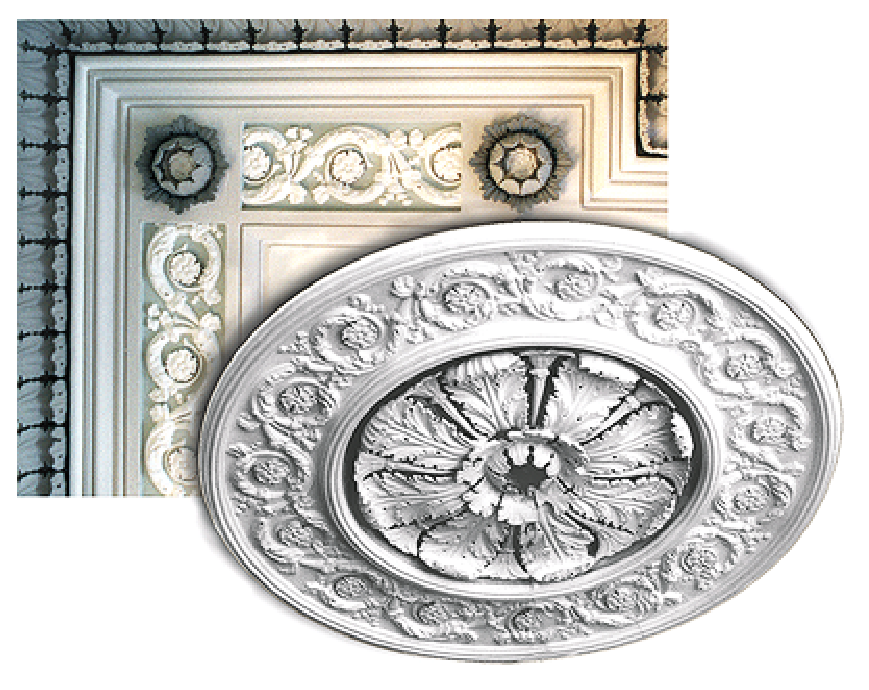
\includegraphics[width=0.85\linewidth]{figures/Cornice_and_rose}
\caption{Plaster cornice and ceiling rose at Regency style building}
\label{plaster_cornice}
\end{figure}

For this research we had access to the prestigious Jackson ornament collection provided by our partner the Regency Town House \cite{rth_2015}. This collection comprises of architectural plaster and composition mouldings used for decorating wall and ceiling spaces. This included architectural elements such as coving, ceiling roses, corbels or panelling. Figure \ref{plaster_cornice} shows an example of a plaster cornice and ceiling rose with a Regency style.  The collection includes reverse cut and positive hardwood and soft wood blocks. It was assembled by the ornamental firm George Jackson and Sons through the 19th and 20th centuries.

The firm Jackson and Sons, founded in 1780 was key in revolutionising the way in which relief decoration was created. They introduced the use of composition plaster into England. Composition plaster differs from traditional plaster as it is produced by a mixture of ingredients, such as chalk, glue, linseed oil and resin \cite{Thornton_1994}. The composition mouldings were formed by using wooden moulds which were carved with extraordinary delicacy and precision (as shown in figure \ref{composite_mould}). The use of wooden moulds meant that the plaster could be prefabricated as opposed to created on site.

\begin{figure}[h]
\centering
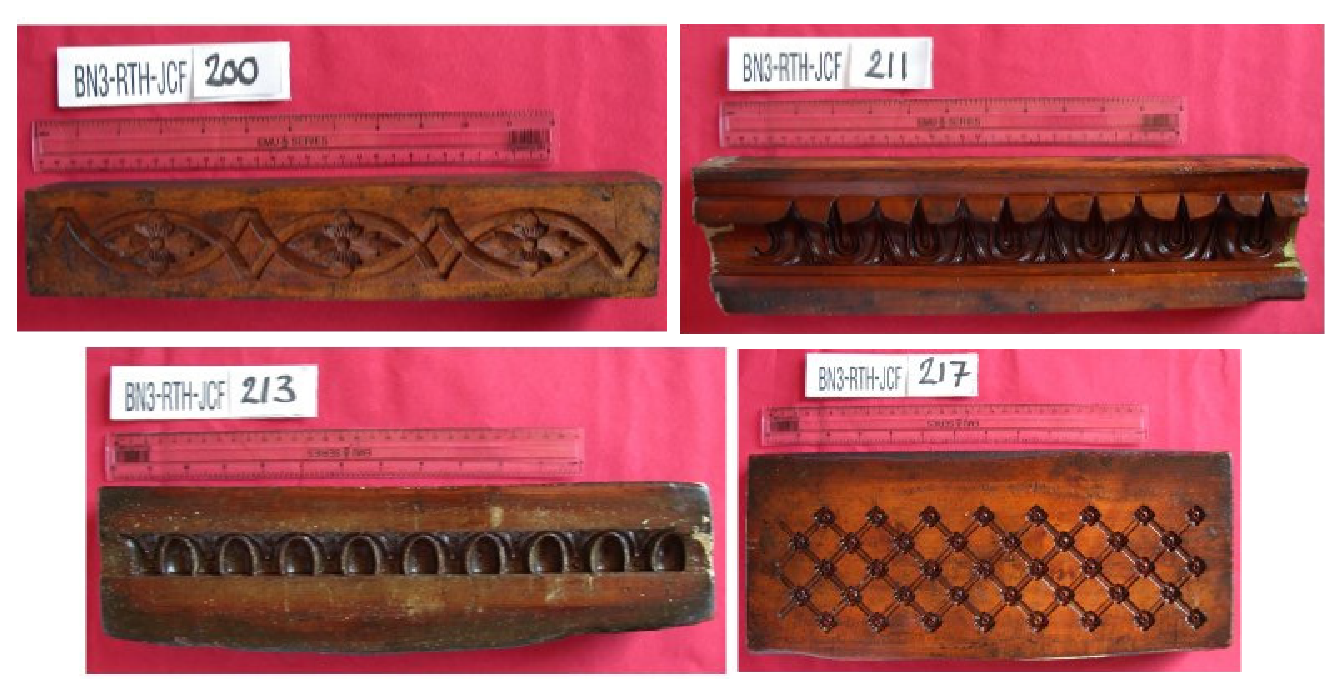
\includegraphics[width=0.85\linewidth]{figures/regency3}
\caption{Example of wooden moulds for plaster and composite plaster mouldings from the Jackson architectural ornament collection.}
\label{composite_mould}
\end{figure}

The vocabulary of motifs and patterns of Regency plasterers was influenced by Neo-Classical motifs. The more important the room, the heavier and more profuse the moulded ornamentation was. Figure \ref{patterns_regency} illustrates some commonly used patterns, including:
\begin{itemize}
\item Anthemion and palmette moulding: pattern comprising alternating palmette and anthemion motifs. The term anthemion comes from the Greek term for \emph{flower}. The palmette is a motif resembling a stylized erect leaf divided into lobes, in the form of a fan or palm leaf, often supported by spirals.
\item Egg and dart moulding: pattern of egg-shaped motif alternating with dartlike motif.
\item Bead and reel moulding: pattern with disks alternating singly or in pairs with oblong beads.
\item Fret moulding: Patterns consisting of repeated, linear, geometrical shapes, usually angular, in a continuous band. 
\end{itemize}

\begin{figure}[h]
\centering
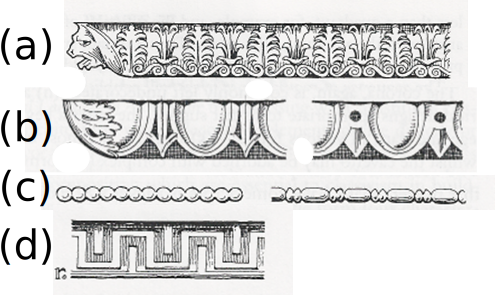
\includegraphics[width=0.85\linewidth]{figures/patterns}
\caption{Patterns commonly used in Regency style mouldings in household interiors. a) pattern with anthemion and palmette motif; b) egg and dart; c) bead and reel; and d) fret pattern \cite{chitham_classical_2005}}
\label{patterns_regency}
\end{figure}

The use of ornament declined after the 1920s following the Modernist Movement. This movement dictated the omission of any superfluous decorations on architectural elements; instead form following only functional requirements. However, towards the end of 1960s there was a resurge of interest on the conservation and preservation of historical buildings. This interest has continued until today, in particular in areas where there is a large concentration of architecture with a particular historical style decorated with ornament. The seafront area of the city of Brighton and Hove, in the South East of the England, is an example of an area with a distinctive Regency style of buildings (see figure 2). Hence, the interest in the use of plaster mouldings to decorate architectural elements both in interior and exterior of buildings remains high. It should be noted that the production of plaster mouldings for these purposes has remained mainly an artisan activity where methods developed by Jackson and Sons and other contemporaries are still in use today.

The Jackson collection is complemented by an existent database (?) with basic information such as�.




\section{Design of ontology to document architectural moulding collection} 
include data we have to describe the current mouldings (based in CIDOC-CRM and Getty AAT thesarus). 

\section{Shape analysis method} 

Describing Ran's implemented method

\section{Results and testing} 

Testing on current scanned shapes 

\section{Conclusions and further work} 

\section*{Acknowledgment}
The research leading to these results has received funding from the Engineering and the Physical Sciences Research Council (EPSRC) under grant agreement No. EP/L006685/1. The authors would like to thank the Regency Town House for providing access to the Jackson ornament collection and relevant expertise for conducting the research.

% trigger a \newpage just before the given reference
% number - used to balance the columns on the last page
% adjust value as needed - may need to be readjusted if
% the document is modified later
%\IEEEtriggeratref{8}
% The "triggered" command can be changed if desired:
%\IEEEtriggercmd{\enlargethispage{-5in}}

% references section

% can use a bibliography generated by BibTeX as a .bbl file
% BibTeX documentation can be easily obtained at:
% http://www.ctan.org/tex-archive/biblio/bibtex/contrib/doc/
% The IEEEtran BibTeX style support page is at:
% http://www.michaelshell.org/tex/ieeetran/bibtex/
%\bibliographystyle{IEEEtran}
% argument is your BibTeX string definitions and bibliography database(s)
%\bibliography{IEEEabrv,../bib/paper}
%
% <OR> manually copy in the resultant .bbl file
% set second argument of \begin to the number of references
% (used to reserve space for the reference number labels box)
\bibliographystyle{IEEEtran}
\bibliography{IEEEfull,mybibfile}



% that's all folks
\end{document}


